% Options for packages loaded elsewhere
\PassOptionsToPackage{unicode}{hyperref}
\PassOptionsToPackage{hyphens}{url}
%
\documentclass[
]{article}
\usepackage{amsmath,amssymb}
\usepackage{iftex}
\ifPDFTeX
  \usepackage[T1]{fontenc}
  \usepackage[utf8]{inputenc}
  \usepackage{textcomp} % provide euro and other symbols
\else % if luatex or xetex
  \usepackage{unicode-math} % this also loads fontspec
  \defaultfontfeatures{Scale=MatchLowercase}
  \defaultfontfeatures[\rmfamily]{Ligatures=TeX,Scale=1}
\fi
\usepackage{lmodern}
\ifPDFTeX\else
  % xetex/luatex font selection
\fi
% Use upquote if available, for straight quotes in verbatim environments
\IfFileExists{upquote.sty}{\usepackage{upquote}}{}
\IfFileExists{microtype.sty}{% use microtype if available
  \usepackage[]{microtype}
  \UseMicrotypeSet[protrusion]{basicmath} % disable protrusion for tt fonts
}{}
\makeatletter
\@ifundefined{KOMAClassName}{% if non-KOMA class
  \IfFileExists{parskip.sty}{%
    \usepackage{parskip}
  }{% else
    \setlength{\parindent}{0pt}
    \setlength{\parskip}{6pt plus 2pt minus 1pt}}
}{% if KOMA class
  \KOMAoptions{parskip=half}}
\makeatother
\usepackage{xcolor}
\usepackage[margin=1in]{geometry}
\usepackage{graphicx}
\makeatletter
\def\maxwidth{\ifdim\Gin@nat@width>\linewidth\linewidth\else\Gin@nat@width\fi}
\def\maxheight{\ifdim\Gin@nat@height>\textheight\textheight\else\Gin@nat@height\fi}
\makeatother
% Scale images if necessary, so that they will not overflow the page
% margins by default, and it is still possible to overwrite the defaults
% using explicit options in \includegraphics[width, height, ...]{}
\setkeys{Gin}{width=\maxwidth,height=\maxheight,keepaspectratio}
% Set default figure placement to htbp
\makeatletter
\def\fps@figure{htbp}
\makeatother
\setlength{\emergencystretch}{3em} % prevent overfull lines
\providecommand{\tightlist}{%
  \setlength{\itemsep}{0pt}\setlength{\parskip}{0pt}}
\setcounter{secnumdepth}{-\maxdimen} % remove section numbering
\usepackage{booktabs}
\usepackage{longtable}
\usepackage{array}
\usepackage{multirow}
\usepackage{wrapfig}
\usepackage{float}
\usepackage{colortbl}
\usepackage{pdflscape}
\usepackage{tabu}
\usepackage{threeparttable}
\usepackage{threeparttablex}
\usepackage[normalem]{ulem}
\usepackage{makecell}
\usepackage{xcolor}
\ifLuaTeX
  \usepackage{selnolig}  % disable illegal ligatures
\fi
\usepackage{bookmark}
\IfFileExists{xurl.sty}{\usepackage{xurl}}{} % add URL line breaks if available
\urlstyle{same}
\hypersetup{
  pdftitle={Adult Children Caregivers Analysis},
  pdfauthor={Anna Bokun},
  hidelinks,
  pdfcreator={LaTeX via pandoc}}

\title{Adult Children Caregivers Analysis}
\author{Anna Bokun}
\date{March 04, 2025}

\begin{document}
\maketitle

{
\setcounter{tocdepth}{2}
\tableofcontents
}
\subsection{Introduction}\label{introduction}

This document analyzes the characteristics of Mexican-American adult
child caregivers from the Hispanic Established Populations for
Epidemiologic Study of the Elderly (HEPESE) Wave 7 dataset (2010-2011).
The analysis focuses specifically on adult children who provide care to
their aging parents, examining different groups based on co-residence
and household headship patterns.

\subsection{Methodology}\label{methodology}

We examine three distinct groups of adult children caregivers:

\begin{enumerate}
\def\labelenumi{\arabic{enumi}.}
\tightlist
\item
  \textbf{Co-residing adult children caregivers}: Adult children who
  live in the same household as their parent care recipients
\item
  \textbf{Adult children who moved in with parents (general)}: Adult
  children who moved in with their parents without specifying caregiving
  as the primary reason
\item
  \textbf{Adult children who moved in for caregiving}: Adult children
  who moved in specifically to provide care to their parents
\end{enumerate}

For each group, we analyze demographic characteristics, socioeconomic
status, health status, caregiving intensity, and financial strain.

\subsection{Results}\label{results}

\subsubsection{Table 1: Characteristics of All Co-residing Adult
Children
Caregivers}\label{table-1-characteristics-of-all-co-residing-adult-children-caregivers}

\begin{table}

\caption{\label{tab:table1}All Co-residing Adult Children Caregivers (N = 191 )}
\centering
\fontsize{12}{14}\selectfont
\begin{tabu} to \linewidth {>{\raggedright}X>{\raggedright}X>{\raggedleft}X>{\raggedleft}X}
\hline
\cellcolor[HTML]{f8f8f8}{\textbf{Characteristic}} & \cellcolor[HTML]{f8f8f8}{\textbf{Category}} & \cellcolor[HTML]{f8f8f8}{\textbf{n}} & \cellcolor[HTML]{f8f8f8}{\textbf{\%}}\\
\hline
 & Female & 123.00 & 64.4\\
\cline{2-4}
\multirow[t]{-2}{*}{\raggedright\arraybackslash \textbf{Gender}} & Male & 68.00 & 35.6\\
\cline{1-4}
 & Early Adulthood (18-44) & 19.00 & 9.9\\
\cline{2-4}
 & Early Retirement (65-75) & 23.00 & 12.0\\
\cline{2-4}
 & Late Middle Age (55-64) & 87.00 & 45.5\\
\cline{2-4}
\multirow[t]{-4}{*}{\raggedright\arraybackslash \textbf{Age group}} & Middle Age (45-54) & 62.00 & 32.5\\
\cline{1-4}
 & Bachelor's+ & 34.00 & 18.3\\
\cline{2-4}
 & HS Graduate & 52.00 & 28.0\\
\cline{2-4}
 & Less than HS & 71.00 & 38.2\\
\cline{2-4}
\multirow[t]{-4}{*}{\raggedright\arraybackslash \textbf{Education}} & Some College & 29.00 & 15.6\\
\cline{1-4}
 & \$10,000-\$19,999 & 43.00 & 25.0\\
\cline{2-4}
 & \$20,000-\$29,999 & 28.00 & 16.3\\
\cline{2-4}
 & \$30,000-\$49,999 & 41.00 & 23.8\\
\cline{2-4}
 & \$50,000+ & 20.00 & 11.6\\
\cline{2-4}
\multirow[t]{-5}{*}{\raggedright\arraybackslash \textbf{Income}} & < \$10,000 & 40.00 & 23.3\\
\cline{1-4}
 & Not on Medicaid & 153.00 & 83.2\\
\cline{2-4}
\multirow[t]{-2}{*}{\raggedright\arraybackslash \textbf{Medicaid status}} & On Medicaid & 31.00 & 16.8\\
\cline{1-4}
 & Married & 66.00 & 35.3\\
\cline{2-4}
\multirow[t]{-2}{*}{\raggedright\arraybackslash \textbf{Marital status}} & Not married & 121.00 & 64.7\\
\cline{1-4}
 & excellent/good & 102.00 & 53.7\\
\cline{2-4}
\multirow[t]{-2}{*}{\raggedright\arraybackslash \textbf{Health status}} & fair/poor & 88.00 & 46.3\\
\cline{1-4}
 & Has financial strain & 30.00 & 15.7\\
\cline{2-4}
\multirow[t]{-2}{*}{\raggedright\arraybackslash \textbf{Financial strain}} & No financial strain & 161.00 & 84.3\\
\cline{1-4}
 & High intensity & 97.00 & 55.4\\
\cline{2-4}
 & Low intensity & 10.00 & 5.7\\
\cline{2-4}
\multirow[t]{-3}{*}{\raggedright\arraybackslash \textbf{Caregiving intensity}} & Moderate intensity & 68.00 & 38.9\\
\cline{1-4}
 & Head of household & 60.00 & 31.4\\
\cline{2-4}
\multirow[t]{-2}{*}{\raggedright\arraybackslash \textbf{Household headship}} & Not head of household & 131.00 & 68.6\\
\cline{1-4}
 & Mean ADL hours/day & 6.29 & NA\\
\cline{2-4}
\multirow[t]{-2}{*}{\raggedright\arraybackslash \textbf{Caregiving hours}} & Mean IADL hours/day & 6.21 & NA\\
\cline{1-4}
 & Parent does not have dementia & 109.00 & 57.1\\
\cline{2-4}
\multirow[t]{-2}{*}{\raggedright\arraybackslash \textbf{Parent cognitive status}} & Parent has dementia & 82.00 & 42.9\\
\hline
\multicolumn{4}{l}{\rule{0pt}{1em}\textit{Note: }}\\
\multicolumn{4}{l}{\rule{0pt}{1em}Data source: HEPESE Wave 7 (2010-2011)}\\
\end{tabu}
\end{table}

\subsubsection{Table 2: Characteristics of Adult Children Who Moved In
with Parents
(General)}\label{table-2-characteristics-of-adult-children-who-moved-in-with-parents-general}

\begin{table}

\caption{\label{tab:table2}Adult Children Who Moved In with Parents - General (N = 21 )}
\centering
\fontsize{12}{14}\selectfont
\begin{tabu} to \linewidth {>{\raggedright}X>{\raggedright}X>{\raggedleft}X>{\raggedleft}X}
\hline
\cellcolor[HTML]{f8f8f8}{\textbf{Characteristic}} & \cellcolor[HTML]{f8f8f8}{\textbf{Category}} & \cellcolor[HTML]{f8f8f8}{\textbf{n}} & \cellcolor[HTML]{f8f8f8}{\textbf{\%}}\\
\hline
 & Female & 18.00 & 85.7\\
\cline{2-4}
\multirow[t]{-2}{*}{\raggedright\arraybackslash \textbf{Gender}} & Male & 3.00 & 14.3\\
\cline{1-4}
 & Late Middle Age (55-64) & 12.00 & 57.1\\
\cline{2-4}
\multirow[t]{-2}{*}{\raggedright\arraybackslash \textbf{Age group}} & Middle Age (45-54) & 9.00 & 42.9\\
\cline{1-4}
 & Bachelor's+ & 3.00 & 14.3\\
\cline{2-4}
 & HS Graduate & 6.00 & 28.6\\
\cline{2-4}
 & Less than HS & 6.00 & 28.6\\
\cline{2-4}
\multirow[t]{-4}{*}{\raggedright\arraybackslash \textbf{Education}} & Some College & 6.00 & 28.6\\
\cline{1-4}
 & \$10,000-\$19,999 & 7.00 & 36.8\\
\cline{2-4}
 & \$20,000-\$29,999 & 5.00 & 26.3\\
\cline{2-4}
 & \$30,000-\$49,999 & 6.00 & 31.6\\
\cline{2-4}
\multirow[t]{-4}{*}{\raggedright\arraybackslash \textbf{Income}} & \$50,000+ & 1.00 & 5.3\\
\cline{1-4}
 & Not on Medicaid & 15.00 & 78.9\\
\cline{2-4}
\multirow[t]{-2}{*}{\raggedright\arraybackslash \textbf{Medicaid status}} & On Medicaid & 4.00 & 21.1\\
\cline{1-4}
 & Married & 8.00 & 38.1\\
\cline{2-4}
\multirow[t]{-2}{*}{\raggedright\arraybackslash \textbf{Marital status}} & Not married & 13.00 & 61.9\\
\cline{1-4}
 & excellent/good & 14.00 & 66.7\\
\cline{2-4}
\multirow[t]{-2}{*}{\raggedright\arraybackslash \textbf{Health status}} & fair/poor & 7.00 & 33.3\\
\cline{1-4}
\textbf{Financial strain} & No financial strain & 21.00 & 100.0\\
\cline{1-4}
 & High intensity & 9.00 & 60.0\\
\cline{2-4}
 & Low intensity & 1.00 & 6.7\\
\cline{2-4}
\multirow[t]{-3}{*}{\raggedright\arraybackslash \textbf{Caregiving intensity}} & Moderate intensity & 5.00 & 33.3\\
\cline{1-4}
 & Head of household & 12.00 & 57.1\\
\cline{2-4}
\multirow[t]{-2}{*}{\raggedright\arraybackslash \textbf{Household headship}} & Not head of household & 9.00 & 42.9\\
\cline{1-4}
 & Mean ADL hours/day & 9.46 & NA\\
\cline{2-4}
\multirow[t]{-2}{*}{\raggedright\arraybackslash \textbf{Caregiving hours}} & Mean IADL hours/day & 6.11 & NA\\
\cline{1-4}
 & Parent does not have dementia & 12.00 & 57.1\\
\cline{2-4}
\multirow[t]{-2}{*}{\raggedright\arraybackslash \textbf{Parent cognitive status}} & Parent has dementia & 9.00 & 42.9\\
\hline
\multicolumn{4}{l}{\rule{0pt}{1em}\textit{Note: }}\\
\multicolumn{4}{l}{\rule{0pt}{1em}Data source: HEPESE Wave 7 (2010-2011)}\\
\end{tabu}
\end{table}

\subsubsection{Table 3: Characteristics of Adult Children Who Moved In
for
Caregiving}\label{table-3-characteristics-of-adult-children-who-moved-in-for-caregiving}

\begin{table}

\caption{\label{tab:table3}Adult Children Who Moved In for Caregiving (N = 27 )}
\centering
\fontsize{12}{14}\selectfont
\begin{tabu} to \linewidth {>{\raggedright}X>{\raggedright}X>{\raggedleft}X>{\raggedleft}X}
\hline
\cellcolor[HTML]{f8f8f8}{\textbf{Characteristic}} & \cellcolor[HTML]{f8f8f8}{\textbf{Category}} & \cellcolor[HTML]{f8f8f8}{\textbf{n}} & \cellcolor[HTML]{f8f8f8}{\textbf{\%}}\\
\hline
 & Female & 20.00 & 74.1\\
\cline{2-4}
\multirow[t]{-2}{*}{\raggedright\arraybackslash \textbf{Gender}} & Male & 7.00 & 25.9\\
\cline{1-4}
 & Early Adulthood (18-44) & 1.00 & 3.7\\
\cline{2-4}
 & Early Retirement (65-75) & 1.00 & 3.7\\
\cline{2-4}
 & Late Middle Age (55-64) & 15.00 & 55.6\\
\cline{2-4}
\multirow[t]{-4}{*}{\raggedright\arraybackslash \textbf{Age group}} & Middle Age (45-54) & 10.00 & 37.0\\
\cline{1-4}
 & Bachelor's+ & 6.00 & 23.1\\
\cline{2-4}
 & HS Graduate & 6.00 & 23.1\\
\cline{2-4}
 & Less than HS & 6.00 & 23.1\\
\cline{2-4}
\multirow[t]{-4}{*}{\raggedright\arraybackslash \textbf{Education}} & Some College & 8.00 & 30.8\\
\cline{1-4}
 & \$10,000-\$19,999 & 6.00 & 30.0\\
\cline{2-4}
 & \$20,000-\$29,999 & 3.00 & 15.0\\
\cline{2-4}
 & \$30,000-\$49,999 & 6.00 & 30.0\\
\cline{2-4}
 & \$50,000+ & 1.00 & 5.0\\
\cline{2-4}
\multirow[t]{-5}{*}{\raggedright\arraybackslash \textbf{Income}} & < \$10,000 & 4.00 & 20.0\\
\cline{1-4}
 & Not on Medicaid & 24.00 & 88.9\\
\cline{2-4}
\multirow[t]{-2}{*}{\raggedright\arraybackslash \textbf{Medicaid status}} & On Medicaid & 3.00 & 11.1\\
\cline{1-4}
 & Married & 14.00 & 53.8\\
\cline{2-4}
\multirow[t]{-2}{*}{\raggedright\arraybackslash \textbf{Marital status}} & Not married & 12.00 & 46.2\\
\cline{1-4}
 & excellent/good & 17.00 & 63.0\\
\cline{2-4}
\multirow[t]{-2}{*}{\raggedright\arraybackslash \textbf{Health status}} & fair/poor & 10.00 & 37.0\\
\cline{1-4}
 & Has financial strain & 6.00 & 22.2\\
\cline{2-4}
\multirow[t]{-2}{*}{\raggedright\arraybackslash \textbf{Financial strain}} & No financial strain & 21.00 & 77.8\\
\cline{1-4}
 & High intensity & 18.00 & 69.2\\
\cline{2-4}
\multirow[t]{-2}{*}{\raggedright\arraybackslash \textbf{Caregiving intensity}} & Moderate intensity & 8.00 & 30.8\\
\cline{1-4}
 & Head of household & 4.00 & 14.8\\
\cline{2-4}
\multirow[t]{-2}{*}{\raggedright\arraybackslash \textbf{Household headship}} & Not head of household & 23.00 & 85.2\\
\cline{1-4}
 & Mean ADL hours/day & 8.05 & NA\\
\cline{2-4}
\multirow[t]{-2}{*}{\raggedright\arraybackslash \textbf{Caregiving hours}} & Mean IADL hours/day & 8.04 & NA\\
\cline{1-4}
 & Parent does not have dementia & 15.00 & 55.6\\
\cline{2-4}
\multirow[t]{-2}{*}{\raggedright\arraybackslash \textbf{Parent cognitive status}} & Parent has dementia & 12.00 & 44.4\\
\hline
\multicolumn{4}{l}{\rule{0pt}{1em}\textit{Note: }}\\
\multicolumn{4}{l}{\rule{0pt}{1em}Data source: HEPESE Wave 7 (2010-2011)}\\
\end{tabu}
\end{table}

\subsection{Comparing Financial Strain Across
Groups}\label{comparing-financial-strain-across-groups}

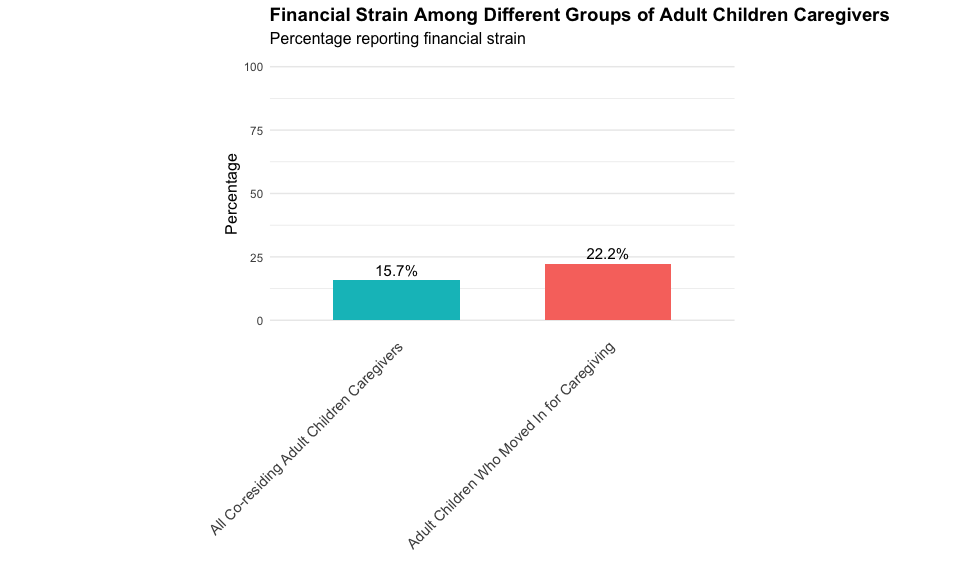
\includegraphics{Adult-Children-Caregivers-Analysis_files/figure-latex/financial-strain-1.pdf}

\subsection{Comparing Caregiving Hours Across
Groups}\label{comparing-caregiving-hours-across-groups}

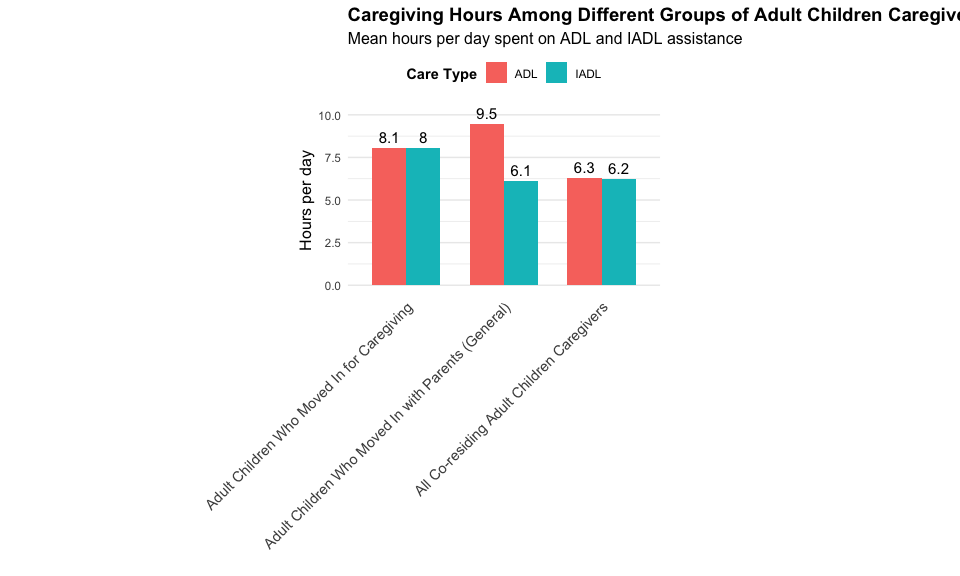
\includegraphics{Adult-Children-Caregivers-Analysis_files/figure-latex/caregiving-hours-1.pdf}

\subsection{Discussion}\label{discussion}

This analysis reveals several important patterns among adult children
caregivers:

\begin{enumerate}
\def\labelenumi{\arabic{enumi}.}
\item
  \textbf{Financial strain:} Adult children who moved in specifically
  for caregiving reasons experience higher rates of financial strain
  compared to caregivers who co-reside without discerning who moved in
  with whom (i.e., Table 1) (22.2\% vs 15.7\%).
\item
  \textbf{Caregiving intensity:} The data shows variation in caregiving
  intensity across different groups. Those who moved in specifically for
  caregiving spent more hours on caregiving tasks, relative to
  caregivers who co-reside without discerning who moved in with whom
  (8.04-8.05 ADL/IADL hours vs 6.21-6.29 ADL/IADL hours).
\item
  \textbf{Demographic differences:} There are notable demographic
  differences between adult children who moved in specifically for
  caregiving versus those who co-reside for other reasons, particularly
  in terms of gender distribution, marital status, and economic
  resources. For example, 11.1\% of adult children who moved in for
  caregiving reasons report participating in Medicaid, vs 21.1\% who
  moved in more generally, and 16.8\% for those who co-reside without
  discerning who moved in with whom.
\item
  \textbf{Household headship:} Among adult children who moved in
  specifically for caregiving reasons, 85.2\% are not the HOH vs 42.9\%
  for adult children who moved in for general reasons. The pattern of
  household headship varies across groups, which may have implications
  for financial decision-making, resource allocation, and caregiver
  autonomy within the household.
\end{enumerate}

\subsection{Limitations}\label{limitations}

Several limitations should be noted when interpreting these results:

\begin{enumerate}
\def\labelenumi{\arabic{enumi}.}
\item
  The data is cross-sectional, limiting our ability to conduct analyses
  over time and to establish causal relationships between co-residence
  patterns and financial strain.
\item
  The sample sizes for some subgroups are prohibitively small (n
  \textless{} 30), which affects the reliability of estimates.
\item
  The HEPESE data is specific to Mexican-Americans in southwestern
  states and may not generalize to other Latino populations or regions.
\item
  Self-reported measures of financial strain and living arrangements may
  be subject to recall bias or social desirability effects.
\end{enumerate}

\end{document}
